%!TEX program = lualatex
\documentclass[11pt]{article}
\usepackage[a4paper, margin=1in, includehead]{geometry}
\geometry{a4paper} 
\usepackage[table, svgnames, dvipsnames]{xcolor}
\usepackage{makecell, cellspace, caption}
\usepackage[utf8]{inputenc}
\usepackage{textcomp}
\usepackage[most]{tcolorbox}
\usepackage{enumitem}
\usepackage{multicol}
\usepackage{graphicx} 
\usepackage{titling}
\usepackage{fancyhdr}
\usepackage{tabularray}
\pagestyle{fancy}
\fancyhf{}
\fancyhfoffset[L]{1cm} % left extra length
\fancyhfoffset[R]{1cm} % right extra length
\rhead{\textbf{\textit{Page-\thepage}}}
\lhead{\textbf{\textit{Software Requirements Specification for PedalPal}}}
\cfoot{}
\usepackage{amsmath,amssymb}  
\usepackage{bm}  
\usepackage[pdftex,bookmarks,colorlinks,breaklinks]{hyperref}  
\hypersetup{linkcolor=black,citecolor=black,filecolor=black,urlcolor=blue} % black links, for printed output
\usepackage{memhfixc} 
\usepackage{pdfsync}  
\usepackage{fancyhdr}
\usepackage{lmodern}
\usepackage{wrapfig}
\usepackage[page,toc,titletoc,title]{appendix}

\usepackage{fontspec}
\setmainfont{Arial}

\pagestyle{fancy}

\usepackage{titlesec}
\begin{document}
\begin{titlingpage}
\begin{flushright}
    \rule{16cm}{5pt}\vskip1cm
    \textbf{{\fontsize{30}{36}\selectfont Design Document}\\\vspace{1cm}\huge{for}\\\vspace{1cm}\Huge{PedalPal}\\ \vspace{1.5cm}\LARGE{Version 1.0}\\\vspace{1cm}\LARGE{Prepared by}}
\end{flushright}
\vspace{1.0cm}
\large{\begin{tabular*}{\columnwidth}{@{\extracolsep{\stretch{1}}}*{3}{c}@{}}
    \Large{\textbf{Group \# 4}} & & \Large{\textbf{Group Name: Bit Brewers}} \\
    \\
    \textbf{Raghav Manglik} & \textbf{220854} & \href{mailto:raghavkmanglik@gmail.com}{raghavkmanglik@gmail.com} \\
    \textbf{Amogh Bhagwat} & \textbf{220288} & \href{mailto:amogh.2004b@gmail.com}{amogh.2004b@gmail.com} \\
    \textbf{Srishti Chandra} & \textbf{221088} & \href{mailto:chandra.srishti2403@gmail.com}{chandra.srishti2403@gmail.com} \\
    \textbf{Wadkar Srujan Nitin} & \textbf{221212} & \href{mailto:srujanwadkar@gmail.com}{srujanwadkar@gmail.com} \\
    \textbf{Anaswar K B} & \textbf{220138} & \href{mailto:anaswarkb013@gmail.com}{anaswarkb013@gmail.com} \\
    \textbf{Khushi Gupta} & \textbf{220531} & \href{mailto:khushi07g@gmail.com}{khushi07g@gmail.com} \\
    \textbf{Ananya Singh Baghel} & \textbf{220136} & \href{mailto:ananyabaghel2004@gmail.com}{ananyabaghel2004@gmail.com} \\
    \textbf{Pathe Nevish Ashok} & \textbf{220757} & \href{mailto:nevu.pathe1234@gmail.com}{nevu.pathe1234@gmail.com} \\
    \textbf{Debraj Karmakar} & \textbf{220329} & \href{mailto:debraj2003jsr@gmail.com}{debraj2003jsr@gmail.com} \\
    \textbf{Kaneez Fatima} & \textbf{220496} & \href{mailto:kaneezfatimamehdi7@gmail.com}{kaneezfatimamehdi7@gmail.com} \\
    
\end{tabular*}}

\vspace{1.5cm}
\begin{center}
\large{
\begin{tabular}{l l}
    \textbf{Course:} & \textbf{CS253} \\
    \textbf{Mentor TA:} & \textbf{Mr. Bharat} \\
    \textbf{Instructor:} & \textbf{Prof. Indranil Saha} \\
    \textbf{Date:} & \textbf{February 9, 2024}
\end{tabular}
}
\end{center}
\end{titlingpage}

\titleformat{name=\section}[block]
  {\sffamily\LARGE}
  {}
  {0pt}
  {\colorsectionx}
\titlespacing*{\section}{0pt}{\baselineskip}{\baselineskip}
\newcommand{\colorsectionx}[1]{\colorbox{gray!120}{\parbox{\dimexpr\textwidth-2\fboxsep}{\color{white} \centering \huge{\textbf{Contents}}}}}

\tableofcontents

\newpage
\titleformat{name=\section}[block]
  {\sffamily\LARGE}
  {}
  {0pt}
  {\colorsection}
\titlespacing*{\section}{0pt}{\baselineskip}{\baselineskip}

\newcommand{\colorsection}[1]{\colorbox{gray!120}{\parbox{\dimexpr\textwidth-2\fboxsep}{\color{white}\huge{\textbf\thesection. }\ #1}}}

\section{\centering{\textbf{Revisions}}}
% \begin{center}
% \begin{tabular}{|c|c|c|c|}
%     \hline
%     \rowcolor{Gainsboro!60}
%     \textbf{Version} & \textbf{Primary Author(s)} & \textbf{Description of Version} & \textbf{Date Completed} \\
%     \hline
%     \makecell{v1.0} & \makecell{Raghav Manglik \\ Amogh Bhagwat \\ Srishti Chandra \\ Wadkar Srujan Nitin \\ Pathe Nevish Ashok \\ Debraj Kamakar \\ Khushi Gupta \\ Ananya Baghel \\ Anaswar K B \\ Kaneez Fatima \\} & \makecell{First version of the Software \\ Requirement Specification \\ (SRS) Document} & \makecell{25/01/23} \\
%     \hline
% \end{tabular}
% \end{center}

\newpage
\section{\centering{\textbf{Context Design}}}
\subsection{Context Model}

\subsection{Human Interface Design}
\subsubsection{Login and Registration Pages}
\begin{figure}[h]
    \centering    
    \includegraphics[scale=0.35]{ui-images/Login.png}
    \hspace{30pt}
    \includegraphics[scale=0.35]{ui-images/Register.png}
    \hspace{30pt}
    \includegraphics[scale=0.35]{ui-images/ResetPassword.png}
\end{figure}
\begin{figure}[h]
    \centering    
    \includegraphics[scale=0.1]{ui-images/PhoneOTP.png}
    \hspace{20pt}
    \includegraphics[scale=0.35]{ui-images/EmailOTP.png}
    \hspace{20pt}
    \includegraphics[scale=0.1]{ui-images/AccountSuccess.png}
\end{figure}

\subsubsection{Booking a Ride}
\begin{center}
\begin{tabular}{ccc}
    \includegraphics[scale=0.35]{ui-images/Dashboard.png} &
    \includegraphics[scale=0.35]{ui-images/HubSelection.png} &
    \includegraphics[scale=0.1]{ui-images/BookRideSubscribed.png} \\
    \includegraphics[scale=0.35]{ui-images/QR.png} & \includegraphics[scale=0.1]{ui-images/ActiveRide.png} & \includegraphics[scale=0.1]{ui-images/RideOver.png}
\end{tabular}
\end{center}

\subsubsection{User Feedback}
\begin{center}
\begin{tabular}{ccc}
    \includegraphics[scale=0.1]{ui-images/CycleIssues.png} & \includegraphics[scale=0.1]{ui-images/IssueDescription.png} & \includegraphics[scale=0.1]{ui-images/FeedbackSubmission.png}
\end{tabular}
\end{center}

\subsubsection{Subscription Model}
\begin{center}
    \begin{tabular}{cc}
        \includegraphics[scale=0.1]{ui-images/BookRideUnsubscribed.png} & \includegraphics[scale=0.1]{ui-images/Advertisement.png}
    \end{tabular}
\end{center}

\subsubsection{Settings and Analytics View}
\begin{center}
\begin{tabular}{ccc}
    \includegraphics[scale=0.36]{ui-images/Navbar.png} & \includegraphics[scale=0.1]{ui-images/Wallet.png} & \includegraphics[scale=0.275]{ui-images/History.png}
\end{tabular}
\begin{tabular}{cc}
\includegraphics[scale=0.1]{ui-images/Settings.png} & \includegraphics[scale=0.1]{ui-images/Bookings.png}
\end{tabular}
\end{center}

\subsubsection{Admin Interface}
\begin{center}
    \begin{tabular}{c}
        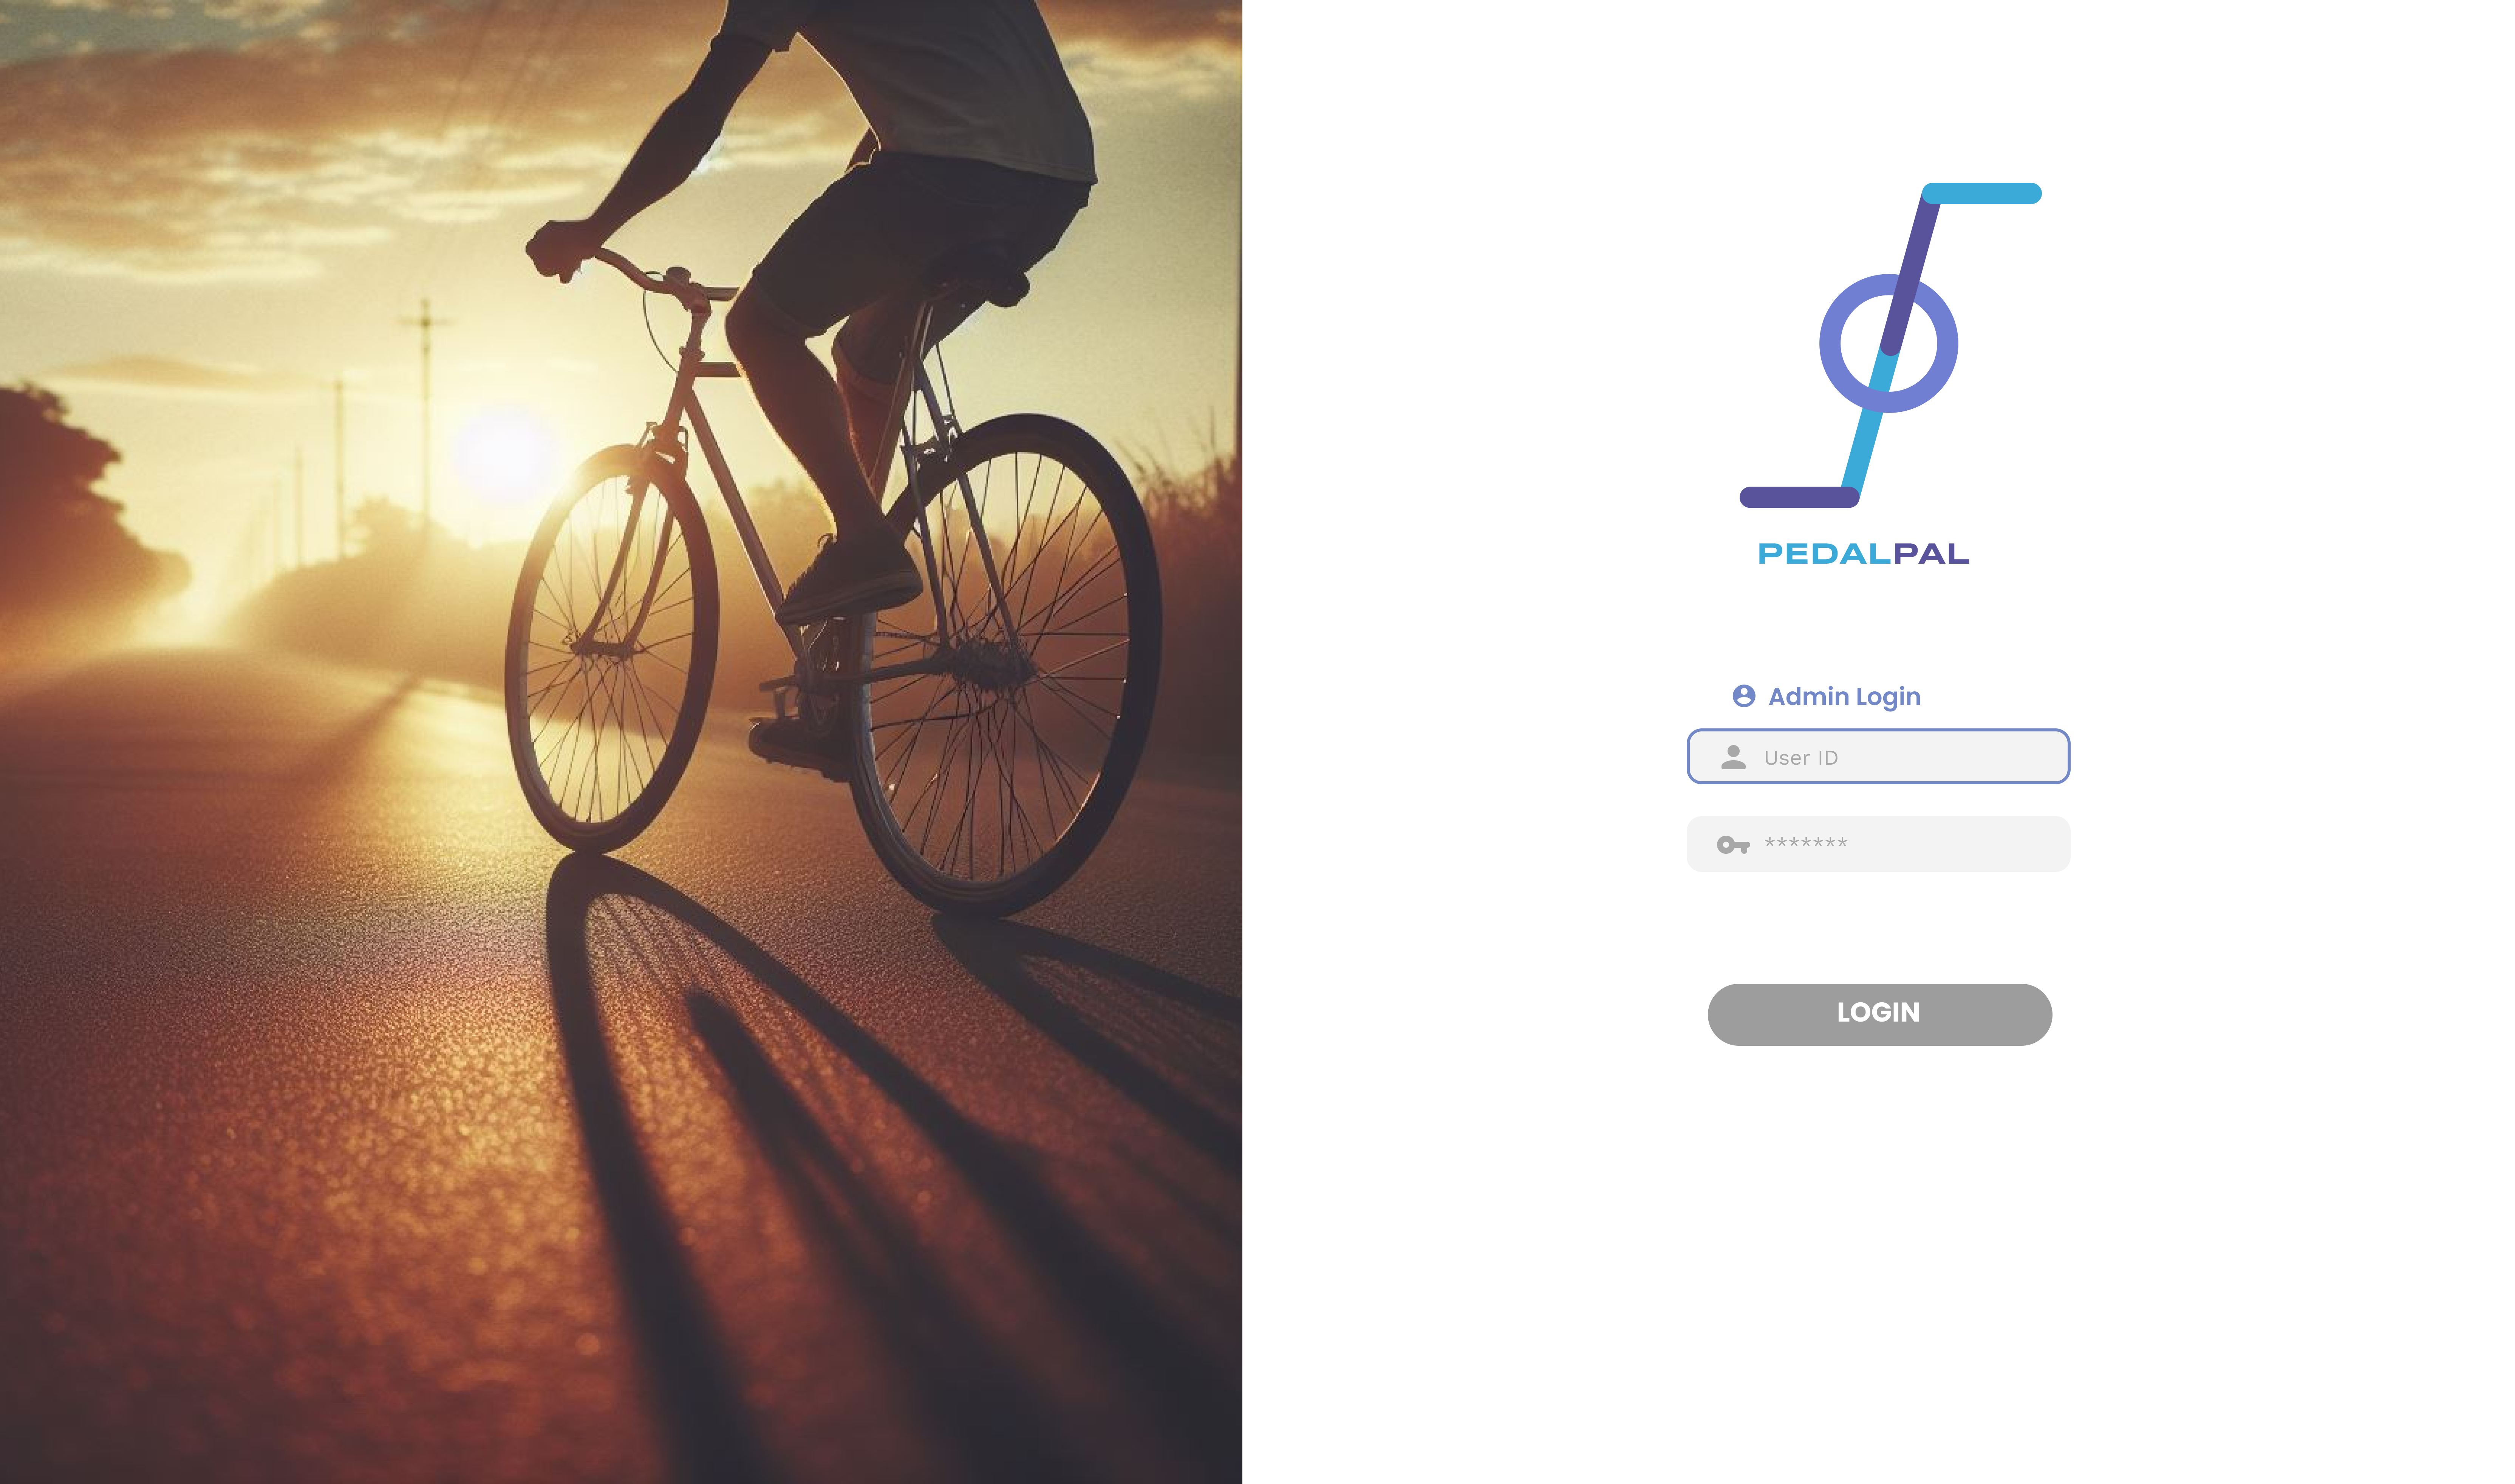
\includegraphics[scale=0.08]{ui-images/AdminLogin.png} \\
        \includegraphics[scale=0.08]{ui-images/AdminDashboard.png}
    \end{tabular}
\end{center}



\newpage
\section{\centering{\textbf{Architecture Design}}}

\newpage
\section{\centering{\textbf{Object Oriented Design}}}
\subsection{Use Case Diagrams}
Overview of the use cases of PedalPal is as follows
\begin{center}
  \includegraphics[scale=0.75]{../srs/Overview.png}
    \includegraphics[scale=0.25]{../srs/usecase.png}
\end{center}
The various use cases are as follows
\subsubsection{Use Case 1}
\begin{center}
  \includegraphics[scale=0.5]{../srs/usecase-1.png}
\end{center}

\subsubsection{Use Case 2}
\begin{center}
  \includegraphics[scale=0.5]{../srs/usecase-2.png}
\end{center}

\subsubsection{Use Case 3}
\begin{center}
  \includegraphics[scale=0.5]{../srs/usecase-3.png}
\end{center}

\subsubsection{Use Case 4}
\begin{center}
  \includegraphics[scale=0.5]{../srs/usecase-4.png}
\end{center}

\subsubsection{Use Case 5}
\begin{center}
  \includegraphics[scale=0.5]{../srs/usecase-5.png}
\end{center}

\subsubsection{Use Case 6}
\begin{center}
  \includegraphics[scale=0.5]{../srs/usecase-6.png}
\end{center}

\subsection{Class Diagrams}

\subsection{Sequence Diagrams}

\subsection{State Diagrams}
\subsubsection{Overall state diagram}
\begin{center}
  \includegraphics[scale=0.125]{state-diagram-images/overall.png}
\end{center}

\newpage
\section{\centering{\textbf{Project Plan}}}

\newpage
\section{\centering{\textbf{Other Details}}}

\newpage
\appendixpageoff
\begin{appendices}

\section{\centering{\textbf{Group Log}}}
% \begin{tabular}{|p{1cm}|p{2cm}|p{2cm}|p{2cm}|p{6.75cm}|}
% \hline
% \makecell{\textbf{S.No}} & \makecell{\textbf{Date}} & \makecell{\textbf{Timings}} & \makecell{\textbf{Venue}} & \makecell{\textbf{Description}} \\
% \hline
% \makecell{1} & \makecell{07/01/2024} & \makecell{14:00\\ to \\16:00} & \makecell{RM \\Building} & \makecell{Brain-stormed various possible \\ prospective ideas for the project. \\ Main ideas presented were: \\ Bicycle Rental Services \\ Hall Management \\ Used goods Buy/Sell Portal} \\
% \hline
% \makecell{2} & \makecell{09/01/2024} & \makecell{14:30\\to\\17:00} & \makecell{Google\\ Meet} & \makecell{Finalized the idea for the project and \\ discussed various aspects of it.} \\
% \hline
% \makecell{3} & \makecell{11/01/2024} & \makecell{22:00\\to\\00:00} & \makecell{Google\\Meet} & \makecell{Studied the SRS template given and \\ distributed the work amongst the team \\ members.} \\
% \hline
% \makecell{4} & \makecell{17/01/2024} & \makecell{21:00\\to\\21:30} & \makecell{Google\\Meet} & \makecell{First meet with the Teaching Assistant \\ Mr. Bharat. Discussed about project \\ and the SRS documentation.} \\
% \hline
% \makecell{5} & \makecell{20/01/2024} & \makecell{15:00\\to\\18:00} & \makecell{Google\\Meet} & \makecell{Brainstorming of final ideas and \\ discussion on use cases, features, \\ data flows.} \\
% \hline
% \makecell{6} & \makecell{21/01/2024} & \makecell{14:00\\to\\15:00} & \makecell{Google\\Meet} & \makecell{Decided to use Django with bootstrap \\ and inline CSS to build the front end \\ part of our application and PostgreSQL \\ as our DBMS.} \\
% \hline
% \makecell{7} & \makecell{22/01/2024} & \makecell{23:00\\to\\00:00} & \makecell{Google\\Meet} & \makecell{Explored more functionalities for the \\ product and progressed with the SRS \\ document.} \\
% \hline
% \makecell{8} & \makecell{25/01/2024} & \makecell{14:00\\to\\17:00} & \makecell{RM\\Building} & \makecell{Finalized the SRS Document and\\completed typesetting in \LaTeX} \\
% \hline
% \end{tabular}
\end{appendices}
\end{document}
